
\chapter{Introduction}

\section{Problem Introduction}
\label{sec:problemintro}
 
 %\section{Zoetermeer and Energy-transition} --> cancelled, start with global warming
 
Due to the urgency that was created by global climate changes, more than a hundred countries, including the Netherlands, are currently creating a joint effort to keep the 1.5\textsuperscript{o} global temperature increase limit compared to pre-industrial temperature level \citep{ClimateFocus2015TheSummary}. This urgency comes from the potential on not only extreme geographical changes \citep{Rogelj2016GeosciencesParis,Fischer2015AnthropogenicExtremes,Mitchell2016RealizingWorld, Vitousek1994BeyondChange, Sheffield2008ProjectedSimulations}, but also   food resources \citep{Nardone2010EffectsSystems,Amundson2006EnvironmentalCattle,Easterling2005AssessingIPCC, Thornton2010ClimateCountries, Kainuma2004AnalysisModel}, diseases \citep{Stewart2017HalfClimate,Wall2011ClimateEnvironment}, economy \citep{Allison2009VulnerabilityFisheries, Helmke2020ProvisionModel}, and the the ecosystem collapse possibility \citep{New2011FourImplications, Scholze2006AEcosystems}. 

\smallskip{}
The Netherlands has turn this critical mission into both legislation (e.g. energy agenda and  climate act) and public cooperation (e.g. climate agreement) \citep{ClimateCouncil2019ClimateAgreement, PlanningOfficefortheLivingEnvronment2019ClimateAchieved, vanderGoot2019FirstPoints, MinistryofEconomicAffairsandClimate2016EnergySupply}. One of the main agendas in these actions is to phase-out gas in 2050 \citep{Beckman2019TheTransition,Deloitte2013EuropeanContents, PlanningOfficefortheLivingEnvronment2019ClimateAchieved}. Despite public skepticism that arose by the end of 2019 \citep{Corder2019DutchMet, Pieters2019SlightGoals, Tidey2019DutchRuling, BBCNewsServices2019NetherlandsEmissions, DutchNews2019DutchOff, FriendsoftheEarth20192050Phase-out}, the Dutch government is confident that this gas phase-out can be successfully implemented with citizen participation, and local municipalities lead \citep{GovernmentoftheNetherlands2019ClimateAffordable}. By the end of 2021, energy-transition policies is anticipated to be ready in every municipality in the Netherlands \citep{ClimateCouncil2019ClimateAgreement,Yuen2019HighlightsAgreement}. 

Still, since uncertainty can emerge under complexity  \citep{Kauffman1993THEEvolution,Kauffman1995AtTrove}, then, policy making can be awry. The government need to use more than assumption to design the optimum possible policy to minimize both national and retail cost as well as minimizing policy sensitivity \citep{ExpertiseCentrumWarmte2019HandreikingAnalyse}. Thus usage of data to drive decision is apparent. Data-driven decision making (DDM) has shown consistent evident on their performances \citep{Brynjolfsson2016TheDecision-making}.

To create a support system for decision making (DSS), both model and data are needed to support decision making \citep{Sage1991DecisionEngineering, Sprague1980ASystems}. The problem that arise from the complexity of policy making shall not only include the decision making support system, but also the selection of model and data \citep{Sage1991DecisionEngineering, Sprague1979BitSystems}. Although the selection of model on energy modeling is vary, more gap can still be found in the area \citep{Hesselink2019AdoptionStudies, Friege2014ModellingReview}. These variation and opportunity can be widen by the information and communication technology (ICT) advancement. For example, to handle data that is too big to be proceed in a traditional approach \citep{Provost2013DataMaking}. 


\smallskip{}
This urgency on an effective energy transition policy from the Netherlands and the opportunity that data brought has open the need to explore the use of big data in the energy-transition policy decision-making. The need for the most optimum policy is dire, and data might be the key to answer uncertainty in the energy transition policy domain. To support policy maker to create their decision, an adapted decision support system concept for energy transition is essential. 

Thus a problem statement is made:

\textit{A need for decision making process concept that can help policy maker to know their needed model and data, for modeler guideline to make more research in the area, and for data provider to know how their data might be needed in the heat transition.}

Then based on this, a research objective is made:

\textit{Support policy maker in their effort to creates policy and modeler and data provider to communicate effectively in order to create the best suited policy for heat transition in the municipality level.}


\subsection{Social relevance}
The research potentially brings new possibility to support heat transition. Starting from one municipality\citep{ZoetermeerMunicipality2019AardgasvrijWonen}, to phase-out gas usage  for more than 50.000 household \citep{ZoetermeerMunicipality2019MunicipalityFigures}. Then gradually, this shall help the possibility to shift 20\% the Netherlands energy usage from natural gas into renewable sources \citep{Eurostat2019Eurostat:Explained, WorldData2019EnergyNetherlands, CBS2019TrendEnerg}.

\smallskip{}
%In addition, compared to a traditional approach, information and communication technology (ICT) that embedded to DDM can also be used as a tool to increase citizen participation in the process \citep{Millard2018OpenMore, Janssen2018InnovatingPrepared, vanVeenstra2017Data-drivenApproach}. Thus can potentially bring trust between policy-maker and the public supported by a transparent platform like the one that \cite {ZoetermeerMunicipality2019OpenZoetermeer} provided. 

%%%%%%%%%%%%%%%%%%%%%%%%%%%%%%%%%%%%%%%%%

\subsection{Scientific relevance}
Energy-transition can be seen as a complex system where to fulfill societal functions, the linkage between elements is necessary \citep{Geels2004FromTheory,VanDam2013Agent-BasedSystems}. The transition itself has been defined as a structured social transformation for a long period \citep{Rotmans2001TransitionsSupply}. It is argued that over a long time of period, this linkage of elements will become more and more blurred.


Thus it is important to see the line and use of both data and model in the process of policy making. By using a data-driven technique into policy making, the uncertainty caused by assumptions can be narrowed \citep{Ameyaw2018SectoralTechnique, Ma2018ForecastingAssumptions}. However, it is needed to map these relationship between data and model that are needed in the policy making to support communication between modeler and data provider.  

%In conclusion, besides a possibility of a higher performances and more inclusive tools for policy-making, a more varying combination of approaches to use data can be explored, and validated.

%%%%%%%%%%%%%%%%%%%%%%%%%%%%%%%%%%%%%%%%%

\subsection{Link to CoSEM program}
Complex system engineering and management (CoSEM) program explore study on creating a design in an emergent environment \citep{TPMStudentportal2019MScCoSEM}. Energy transition is a multidisciplinary and complex system that involves not only technical but also social variables in its problem, including legal, behavior, and economy. Moreover, energy transition has diverse stakeholders with their own interests. Thus creates a multidisciplinary complex problem in which a CoSEM study is needed. In this research stakeholder analysis, socio-technical domain modeling, and market analysis of the system shall be studied. 

%%%%%%%%%%%%%%%%%%%%%%%%%%%%%%%%%%%%%%%%%

\subsection{Proposal Structure}
Section 1.2 the state-of-the-art of data-driven policy-making in the household energy transition, identifies knowledge gaps, then present the main research question. In Chapter 3 the proposed research approach is presented. Furthermore, in chapter 4, a specific research methods and flow diagram is elaborated. Lastly, the research schedule is provided in chapter 5.

\section{Literature research: the concept of policy-making using data-driven tools}
An literature review can be intended to denote the research contribution to the body of knowledge \citep{Hart1998DoingPaperback, Marshall1989B.1999} and provide model on he concept importance \citep{Creswell1994ResearchApproach}. Thus, a literature review is done to explore the use of data-driven policy-making in the energy-transition to find the research gap that exist in the subject as well as their relationship of variables and issues within the system as has been done by \citep{Baumeister1997WritingReviews}. This literature review technique shall focus either on three types of literature review focuses, integration, theoretical, or methodological \citep{Cooper1988OrganizingReviews} depends on the research questions states bellow. 

This literature study shall shows the state of the art of the data driven decision making in the energy transition that has been presented as problem in section \ref{sec:problemintro}. Besides, this literature review shall also be used to construct adopted methodology for the research as taught by  \citep{Ridley2012TheStudents}. 

From the found knowledge gap in this  research, the main question of this research is presented at the end of this chapter.

\subsection{Systematic Literature Review Approach}
A good literature review need to show the properties of academic writing. Thus they need to have a clear and logical approach \citep{Hart1998DoingPaperback}. The literature research shall use \citep{Kitchenham2009SystematicReview, Kitchenham2007GuidelinesEngineering} review method enhanced by  \citep{Jalali2012SystematicSnowballing, Wohlin2014GuidelinesEngineering} methodology on snowballing for several most important founded papers. Moreover, \citep{Levy2006AResearch} method on creating report on literature review shall be used. The planning of \citep{Webster2002Analyzing.} on the research structure is used in this literature research.   
%Based on \citep{Kitchenham2009SystematicReview, Kitchenham2007GuidelinesEngineering,Levy2006AResearch,Webster2002Analyzing.,Jalali2012SystematicSnowballing, Wohlin2014GuidelinesEngineering, Wee2016HowPaper, Brereton2007LessonsDomain, Brocke2009RECONSTRUCTINGPROCESS}, 
A systematic literature review approach that is adapted  (see figure \ref{fig:slr}) from \citep{Kitchenham2007GuidelinesEngineering} is shown in figure \ref{fig:slr}. This approach is used to ensure research the replicability and the appropriate level of quality. 
%https://www.overleaf.com/project/5e36fb4ed8be3e00010b43f6The systematic literature approach review presented by \citep{Kitchenham2007GuidelinesEngineering} is complemented by taking into account \citep{Levy2006AResearch}

\begin{figure}[htbp!]
  \caption{Systematic Literature Review Approach adapted from \citet{Kitchenham2007GuidelinesEngineering,Levy2006AResearch}}
  \centering
  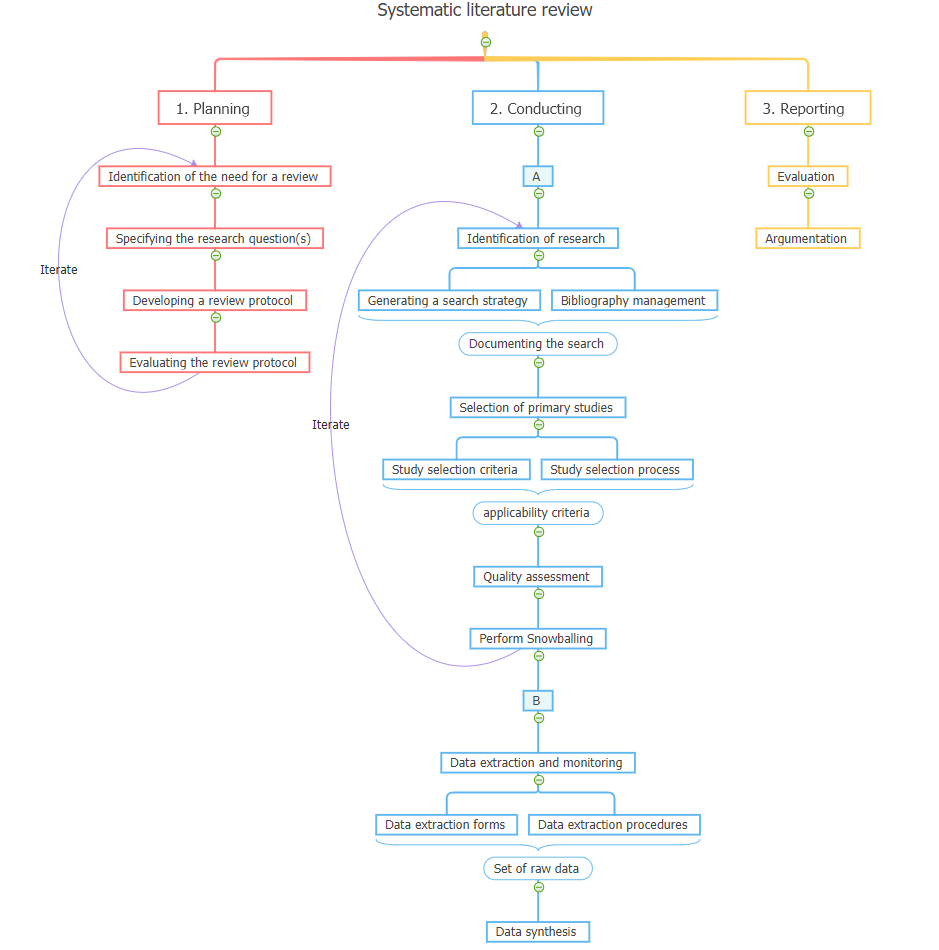
\includegraphics[width=1.0\textwidth]{Images/Decision/Systematic literature review modified.PNG}
   \label{fig:slr}
\end{figure}

Literature research was done using two literature databases, https://scholar.google.nl/ (first five pages based on relevance) and www.scopus.com.

\subsubsection{Literature Search Questions and Keywords}
To find out how far does data-driven decision-making tools have been used on the energy transition policy-making, three questions and keywords are used as follow. 
\begin{itemize}
  \item \textbf{What is data-driven decision making?} Keywords: "data-driven" AND ("policy" OR "decision") AND "making" with document type: review
 % \item \textbf{What kind of variable has been researched using data-driven tools in the energy sector?} Keywords: "data-driven" AND ("model" OR  "tools") AND  "policy" AND "energy" with document type: all
%  \item \textbf{What sector has been researched for data-driven tools in the energy transition domain?} Keywords: "data-driven" AND ("model" OR  "tools") AND  "policy" AND "energy" with document type: all
  \item \textbf{How data-driven tools have been used in the energy transition?} Keywords: "data-driven" AND ("model" OR  "tools") AND  "policy" AND "energy" with document type: all
    \item more about data driven decision making \citep{Diran2019Data-drivenApproach}, look around anneke and janssen
      \item more about model look into  \citep{Hesselink2019AdoptionStudies, Friege2014ModellingReview}
          \item some about policy making framework like    \citep{Farshidi2018ASelection, Sage1991DecisionEngineering, Sprague1980ASystems, Sprague1979BitSystems}
  
\end{itemize}

\subsubsection{Quality Assessment}
To make sure only high-quality papers are used, several requirements are added:
\begin{itemize}
     \item Papers should be published in a scientific journal or at a scientific congress.
    \item Papers are peer-reviewed
\end{itemize}

For the first question, due to the fundamental nature of the issue, one more criterion is added, only five most cited papers are used (minimum of 300 citation per paper).  

\subsubsection{Relevant Concept Check}
Filtered literature then scanned for their relevancy for the literature research questions. Only relevant information shall be documented for further research. Some papers is excluded if they have no relevance to literature research questions. 

\subsubsection{Snowball the Literature}
Additional papers are added based on their relevancy using the snowballing technique. Some vital information that needs to be obtained from their source is gained by snowballing essential sources. 

\subsubsection{Generate Insight}
The state-of-the-art of the knowledge body shall be synthesized using the insight that comes from the literature.

\newpage
\subsection{Literature on the Energy Transition Data-Driven Tools}
Using a systematic literature review approach, 53 papers are studied. A list of papers is shown as follow in the appendix \ref{app_A}.

\subsection{Introduction to Data-Driven Decision Making}

Data-driven decision making is used when traditional data processing is not enough to process the amount of generated data \citep{Provost2013DataMaking}. However, the use of this technique does not warranty effective policy\citep{Marsh200MakingEducation, Wohlstetter2008CreatingFramework}. Effort in data collection is essential to create a proper analysis \citep{Provost2013DataMaking, Marsh200MakingEducation}. Data-driven decision-making technique consists of systematic collection, analysis, examination, and interpretation \citep{Mandinach2012APractice} that is supported by most importantly data analytic thinking \citep{Provost2013DataMaking}. Besides data analysis, these systems can also be used for stakeholder engagement efforts \citep{Janssen2018InnovatingPrepared, Wayman2005InvolvingReflection}.   

Decision support system is a tool or set or tools that support decision making process \citep{Keen1980DecisionAnalysis, Sprague1980ASystems}. As figure \ref{fig:DSS framework}, this tools include the usage of database management system, model management system, then lead to decision management system. 

        \begin{figure}[htbp!]
        \caption{DSS by \citet{Sage1984BehavioralSupport}}
        \centering
            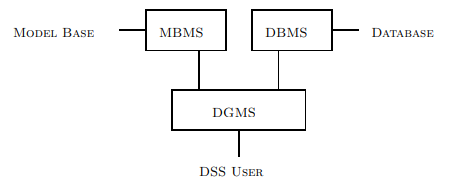
\includegraphics[width=0.5\textwidth]{Images/Decision/DSS by Sage 1991.PNG}
            \label{fig:DSS framework}
        \end{figure}

The need of data and model can be expanded to both qualitative and quantitative decision based. One of the decision model that can be used is the multi criteria decision making. 

\subsection{Data Driven Model usage in Energy Transition}
The DDM making has been widely used in the energy transition policy making as shown in table 1 below. \citep{Zhou2016BigInsights, Nashawi2010ForecastingModel, Yan2019Data-drivenSearch,Bukhsh2018TowardsGrid,Wu2019OptimalApproach,Wang2020ASources,ClimateCouncil2019ClimateAgreement,Singhal2019AResources} created tools to manage power generation using regression analysis. \citep{Guo2019Data-basedStudies,Ma2018ForecastingAssumptions,Mehrtash2018Security-ConstrainedData, Wang2020ASources} manage to forecast the need for power transmission in the electricity sector. This approach was also used by \citep{Zhou2016BigInsights,Godwin2013ClassificationAnalysis,Sharma2019AssessmentFramework} to predict assets managements problems while  \citep{Zhou2016BigInsights,Godwin2013ClassificationAnalysis,Wang2020ASources} predicted operation collaboration problems. 

Market condition \citep{Nashawi2010ForecastingModel, Silvapulle2017NonparametricCountries, Singham2015OptimalLevels, Wu2019OptimalApproach, Khezeli2016Data-drivenResponse} and efficiency \citep{Hong2014DataBuildings, Kontokosta2017ABuildings, Papadopoulos2019GradingData} has also be explored with data driven tools. 

Even complex problem such as demands management \citep{Zhou2016BigInsights,Nashawi2010ForecastingModel,Costanzo2016ExperimentalSystem,Bassamzadeh2017MultiscaleNetworks,Kazmi2016GeneralizableNZEB,Bukhsh2018TowardsGrid, Leurs2016BeyondUnit, Filipe2019Data-drivenStation, Mbuwir2018Self-learningMicrogrid, Khezeli2016Data-drivenResponse}, demands calculation \citep{ONeill2016DevelopmentPerformance, Kontokosta2015ModelingPolicy, Nutkiewicz2017Data-drivenWorkflow, Nutkiewicz2018Data-drivenWorkflow, Biondi2016TheCase, Niemierko2019AData, Ameyaw2018SectoralTechnique, Papadopoulos2017SpatialData, Shah2018RegulatoryBarbuda, Contreras-Ocana2018TractableData, Yu2017PosterUSA, Jia2017PlanningBeijing}, prosumers management \citep{Mbuwir2017BatteryLearning, Mbuwir2018Self-learningMicrogrid, Leurs2016BeyondUnit}, and their storages \citep{Mbuwir2017BatteryLearning, Wu2019OptimalApproach, Shang2020StochasticApproach} are also cases that can be forecasted using DDM. 

Location functionality \citep{Pevec2018AInfrastructure, Lee2016AdoptionSearch-queries, Nutkiewicz2017Data-drivenWorkflow, Papadopoulos2017SpatialData, Wang2020ASources} can also be embedded into the DDM system to help with policy evidence data  \citep{Lee2016AdoptionSearch-queries, Musella2016MappingModels, Dundon2015TheRegulators, Niemierko2019AData} 

%missing
%baldassare 2019, Liu 2019, yuen and karperien 2019 
\begin{table}[htbp!]
    \centering
    \begin{tabular}{c|c|c|c|c|c}
 \hline
  
 \textbf{Usage Type}  
 &   \textbf{Electricity}   
 &   \textbf{Heat} 
 &   \textbf{Fossil}
 &   \textbf{Carbon} \\
    \hline 
    \hline
      Power productions  
      & % electricity
      \cite{Zhou2016BigInsights, Yan2019Data-drivenSearch, Wang2020ASources, Singhal2019AResources, Bukhsh2018TowardsGrid, Wu2019OptimalApproach}
      & % heat
      -
      & % fossil
      \cite{Nashawi2010ForecastingModel}
      & % carbon
      -
 \\  \hline 
      Transmission and distribution   
      & % electricity
      \cite{Ma2018ForecastingAssumptions, Wang2020ASources}
      & % heat
      \cite{Guo2019Data-basedStudies}
      & % fossil
      -
      & % carbon    
      -
%      \cite{Mehrtash2018Security-ConstrainedData}     
\\     \hline 
      Asset management  
     & % electricity
      -
      & % heat
      \cite{Zhou2016BigInsights, Godwin2013ClassificationAnalysis}
      & % fossil
      -
      & % carbon
      -
     % \cite{,,Sharma2019AssessmentFramework}     
      
      \\ \hline 
      Collaborative operation    
     & % electricity
      \cite{Wang2020ASources,Zhou2016BigInsights}
      & % heat
      \cite{Godwin2013ClassificationAnalysis}
      & % fossil
      -
      & % carbon
      -
\\ \hline 
      Demand side management   
     & % electricity
      \cite{Bassamzadeh2017MultiscaleNetworks,Leurs2016BeyondUnit,Filipe2019Data-drivenStation, Zhou2016BigInsights,Khezeli2016Data-drivenResponse,Bukhsh2018TowardsGrid, Mbuwir2018Self-learningMicrogrid}
      & % heat
      \cite{Kazmi2016GeneralizableNZEB}
      & % fossil
      \cite{Nashawi2010ForecastingModel}
      & % carbon
      -
%       \cite{,Costanzo2016ExperimentalSystem,,,, , , , }     
\\ \hline 
      Price forecast    
     & % electricity
      \cite{Wu2019OptimalApproach, Khezeli2016Data-drivenResponse}
      & % heat
      -
      & % fossil
      \cite{Nashawi2010ForecastingModel, Silvapulle2017NonparametricCountries}
      & % carbon
    \cite{Singham2015OptimalLevels}    
\\ \hline 
      Efficiency management    
     & % electricity
      -
      & % heat
      \cite{Hong2014DataBuildings, Kontokosta2017ABuildings}
      & % fossil
      -
      & % carbon
      -
%    \cite{Papadopoulos2019GradingData}     
\\ \hline 
      Demands calculation    
     & % electricity
      \cite{Nutkiewicz2017Data-drivenWorkflow, Nutkiewicz2018Data-drivenWorkflow, Ameyaw2018SectoralTechnique, Shah2018RegulatoryBarbuda, Contreras-Ocana2018TractableData, Jia2017PlanningBeijing}
      & % heat
      \cite{ONeill2016DevelopmentPerformance, Niemierko2019AData}
      & % fossil
      -
      & % carbon
      -
 %               \cite{, Kontokosta2015ModelingPolicy, , Biondi2016TheCase, ,  Papadopoulos2017SpatialData, , , Yu2017PosterUSA, }     
 \\ \hline 
      Prosumer management    
     & % electricity
      \cite{Mbuwir2017BatteryLearning, Mbuwir2018Self-learningMicrogrid, Leurs2016BeyondUnit}
      & % heat
      \cite{Leurs2016BeyondUnit}
      & % fossil
      -
      & % carbon
      -
      
      \\ \hline 
      Storage management    
     & % electricity
      \cite{Mbuwir2017BatteryLearning, Shang2020StochasticApproach,Wu2019OptimalApproach}
      & % heat
      -
      & % fossil
      -
      & % carbon
   -
   
\\ \hline 
      Location management    
     & % electricity
      \cite{Wang2020ASources, Nutkiewicz2017Data-drivenWorkflow}
      & % heat
      -
      & % fossil
      -
      & % carbon
      -
%                \cite{Pevec2018AInfrastructure, Lee2016AdoptionSearch-queries, , Papadopoulos2017SpatialData, }     
\\ \hline 
%      Opinion management    
%     & % electricity
%      \cite{}
%      & % heat
%      & % fossil
%      & % carbon
%                \cite{Lee2016AdoptionSearch-queries, Musella2016MappingModels}     
% \\ \hline 
      Compliance management    
     & % electricity
      -
      & % heat
      \cite{Niemierko2019AData}
      & % fossil
      \cite{Dundon2015TheRegulators}
      & % carbon
      -
 \\
    \hline

    \end{tabular}
    \caption{Data Driven Tools Usage in Energy Transition Policy}
    \label{usage_papers}
\end{table}

\subsection{Research Gap and Main Research Question}
Based on these insights, we can see that DDM has been widely used and proven in various aspects of decision making. However, in this literature, it can be seen that none have integrated their model into a complete energy system. This combination should be done by combining the production, transmission, and consumer side of the system with policy evidence data. 

Moreover, none of this literature combines both central and decentralized in a heating system. This scenario is something that should be explored since a broad spectrum of stakeholders is needed to achieve the 2030 and 2050 target in climate change \citep{GovernmentoftheNetherlands2019ClimateAffordable}.

Furthermore, we can see that the centralized heating system has not been touched much in the literature. This is contradictory to the Netherlands' effort to use their geothermal energy for heating purposes \citep{GovernmentoftheNetherlands2019ClimateAffordable}.

Based on these research gaps, heat transition is chosen in the broad spectrum of energy transition due to the missing links in both the centralized-decentralized system as well as the centralized heating forecasting system. This shall be complemented by geo-location and policy evidence data to forecast public heat demands as well as technology adoption preferences.

Combines with the problem definition in section 1, a research question is formulated \textbf{“How can data and decision making in the energy domain be linked in with the data and model in both technical and social domains?"}


\section{Research Approach and Sub-Questions}

\subsection{Research Approach}
%To answer this “How” question, the characteristic of this question should be analyzed. Looking at this, the problem of a design approach that can also be taken as a problem-solving process \citep{Hevner2004DesignResearch,Johannesson2014AnScience} should be considered. In this kind of approach, the problem should be solved using an artifact. This artifact can be a technical, institutional, process, or combination of any \citep{Johannesson2014AnScience}. The the validation should be done in a study case approach.  

%This design process will include seven sub-step, (1) problem identification and motivation, (2) definition of the objectives for a solution, (3) design and development, (4) demonstration, (5) evaluation, and communication (6) \citep{Peffers2007AResearch}.  

The system shall be analyzed in a study case approach. Study case approach is used in a modest scale of research \citep{Rowley2002UsingResearch} to answer a "how" question about an set of current event where researcher are detached from the system \citep{Yin1994DiscoveringResearch} on either new or inadequate existing theory \citep{Eisenhardt1989BuildingResearch}. In this case, I am using case study for an exploration of the existing theory in a new field. As suggested by \citep{Eisenhardt1989BuildingResearch} this study case will be done in an incremental way where the order shall be divided into smaller tasks as well as iterative, where the design shall be evaluated and remade during the whole design process \citep{Cockburn1998UsingDevelopment}. 

Case study is helpful to give insight to answer an \textbf{explanatory} research using evidence from various sources such as documents, artifacts, interview, or observation \citep{Rowley2002UsingResearch}. The most challenging step that can be induced to a case study is to transform the phenomenon into a piece of research that can be labeled as important.  

As for incremental approach, the advantage of the this approach is that the designer can learn from their previous increment stage \citep{Larman2004AgileLivros}.  This means that any prior increment knowledge can be useful for the next increment. Therefore, it is arguable that the process for the future increase in line can go faster toward the end of the project. This speed is also supported by customer satisfaction on early feedback and active participation \citep{Petersen2009TheDevelopment}. 

This kind of fast interaction will help less miscommunication. And in the end, reduce the time needed for design. This advantage is required for this project because of the high number of stakeholders, client, and colleague in this project as this project will be done in cooperation with several researchers of TNO, Zoetermeer municipality, TU Delft, and one master student. 

%However, this approach also has some problems due to the fast nature of this approach. Since this incremental problem requires high coordination and testing, a tremendous amount of testing data and high coordination effort will be needed \citep{Petersen2009TheDevelopment}. In this research case, this became even more problematic since each engineer will not only handle one project. Therefore, the master student needs to be able to manage this communication and documentation as useful as possible between TU Delft, TNO, and the municipality.

\subsection{Sub-Questions}

To answer the main research question, seven sub-questions that follow the guidelines of design science by \citep{Hevner2004DesignResearch} should be made. In an incremental approach, the problem shall be divided into smaller problems \citep{Cockburn1998UsingDevelopment}. Each sub-question shall be taken as one increment in the design process. After all, sub-question answered, the result shall be used to solve the last increment, the main research question. 
%The first three research questions shall answer the state of the art of the approach (Data-driven policy lab approach), the Netherlands heat transition, as well as the big data availability. The answer from there shall be used to answer the fourth and fifth sub-questions. Then the sixth till eight sub-question shall be answered. After the seventh and eight sub-question explained, the main research question shall be discussed.

These sub-questions are listed as follows.

Comment from TNO: Too much, reduce to number 5 only, but I was talking about testing and stuff, need advice on this.

\begin{enumerate}



    \item Who are the relevant stakeholders in the heat transition in the municipality area?
    \item What are the roles of data driven model (e.g. machine learning, deep learning) to support decision making in the heat transition?
    \item Linked to model usage, how data can be used in the effort to create decision in the heat transition policy?
    \item Linked to the relevant stakeholders in the heat transition in the municipality area, who are the data source of the needed data to be used in the decision support system?
    \item How does decision making process in heat transition policy in the municipality level be translated into a conceptual model using the decision support system approach by defining the relationship between data and model?
    %where they can be added to fill in the blank
    \item How can citizen involvement be included in the decision support conceptual mode scheme? 
    \item To what extent is the conceptual model of decision support in heat transition can be accurate and beneficial for policy maker, data provider, and modeler?
    \item To what extent is the conceptual model of decision support in heat transition can increase citizen participation in the heat transition?
    
    \item [OPTIONAL] What additional data are found to be needed in the case of the selected neighbourhood model using the decision support conceptual model? --> TNO said, better to not include in the proposal, but might be done in a project without timeline restriction
    \item [OPTIONAL] What additional model found beneficial to be made in the case of the selected neighbourhood model using the decision support conceptual model? --> TNO said, better to not include in the proposal, but might be done in a project without timeline restriction

\end{enumerate}

\section{Research Method}
To include both the living lab approach as well as the data-driven technique, a policy lab approach shall be used in this incremental design research. Policy lab is a dedicated structure that derived an innovative method to catch the interaction between policy and its stakeholders in the design process \citep{Fuller2016PublicStates}.  They have been growing all-around European countries like Denmark, French, and the Netherlands \citep{Fuller2016PublicStates,Williamson2015GoverningEducation}. Combined with the data-driven approach, a policy lab approach was proposed by TNO in 2015 \citep{vanVeenstra2017Data-drivenApproach}. 
This approach connects the policy-making cycles, “Predictive \& problem definition”, “Design \& experimentation”, and “Evaluation \& implementation” \citep{Lasswell1951TheOrientation}  with data-driven approach. These cycles were translated into “fore sighting and early warning”, “modeling and simulation”, “monitoring impact and assessments”\citep{vanVeenstra2017Data-drivenApproach}. 
This approach has been adopted by several precedent types of research \citep{Diran2019Data-drivenApproach, Federico2019DesignInnovation, Ibrahim2020UnderstandingAnalytics, Kruyen2018TowardsApproach, Radermacher2019Governing-by-the-numbers/statisticalSociety}. All this literature describes the usage of the policy lab approach in data-driven mechanics. However, this has not evolved enough despite its potential. More frameworks and tools need to be experimented to create a tangible use of this approach. Some addition and adaptation shall be made based on the result of the increment (refer to section 3) in the research.

\subsection{Research Flow Diagram}
The flow diagram of this research is presented in figure \ref{fig:flow}. This flow diagram is made to explain the interrelations between research questions, tools to be used, and how it will be presented in the master thesis chapters.

\begin{figure}[htbp!]
  \caption{Flow Diagram.}
  \centering
  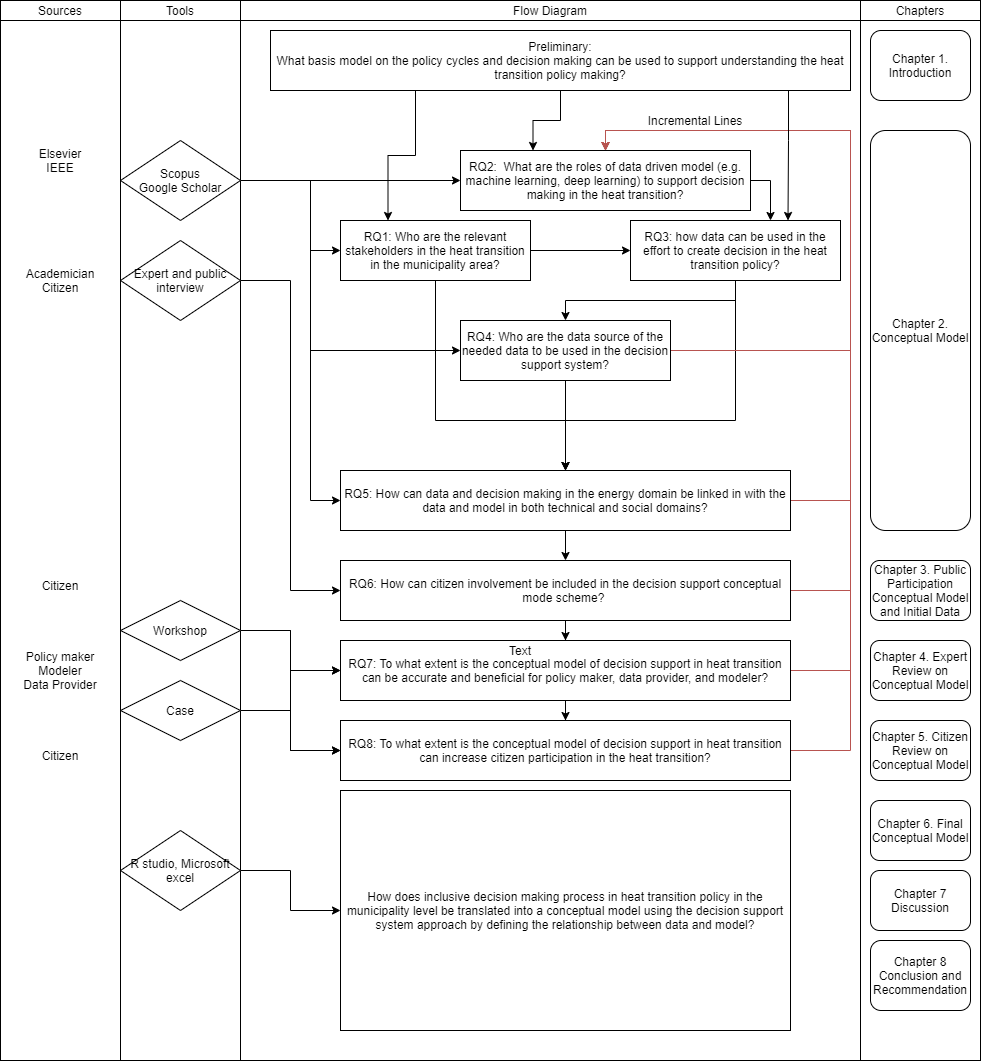
\includegraphics[width=1.2\textwidth]{Images/Flow.png}
   \label{fig:flow}
\end{figure}
 
\subsection{Introduction of the Research}

%In the introduction, three first research questions (see chapter 3) shall be answered. In this introduction, literature research shall be done. The literature research shall be done in the European policy domain within the last ten years. This literature shall be replicable as a clear method will be defined \citep{Wee2016HowPaper}. A systematic approach on literature review shall be used for this (please refer to chapter 2). The advantage of this method is that since this little direct contact will be made with the research object, the result of this stage shall be fast and reproducible easily. Moreover, the usage of knowledge from other shall give the benefit of time. 
%Due to the same reason, the result of the study might not represent the future with the most recent status of the world. However, in this specific case, this disadvantage might not be essential. The cause for this is that this question shall be used to make scenarios in the later stage. Therefore, ten years of prior prediction should be sufficient. 
%For this, access to journal publisher as well as libraries are needed. In case of access is not granted, the literature shall not be used except if the literature is highly cited. In that case, access shall be bought. The search engine that shall be used in this research will be https://www.scopus.com/ and https://scholar.google.nl/ (with limitation of five first pages).  

%All relevant stakeholders in the heat transition are shall be done using literature research as described in the previous sub question. For extra information, the result from the literature research will be validated by expert from TU Delft, TNO, and Zoetermeer municipality. 

\subsection{Heat Transition Decision Making Conceptual Model}

From findings in the literature research, the fourth and fifth sub-question shall be answered with both literature research and interview. The literature research shall provide an idea of the interview question. Then, the question shall be used in the Delphi style interview. 
The advantage of using this method is that a high-quality answer shall be presented based on expert discussion compared to a one-way interview. It is expected that this method will have resulted in unified experts’ opinions that reinforced each other. This process is guaranteed to creating data with high reliability.
Like the previous question, access to the journal publisher as well as the library is needed. Furthermore, access to both academic and policy experts in shall be taken.  The required capability of these experts shall be determined by the number of experiences in their field. Both age and working years shall not be criteria for interview participants. The participant shall enter this interview voluntarily. Between 4 to 8 participants (STILL NEED TO FIND LITERATURE ON NUMBER AND STUFF) are expected to be sufficient to do a proper interview process since Delphi method goes more into quality than quantity \citep{Boulkedid2011UsingReview}.

The interview process shall be in line with the TU Delft data management system as stated by \citep{GrootKormelink-TBM2018ProcessingPrivacy}. All data will be secured in the surf database and should be compliance with European General Data Protection Regulation (GDPR). 

Furthermore, the iteration of the previous sub question shall also be followed in this increment.  

\subsection{Case Selection and Data Collection}

A case should be observed in a bounded context, the unit of analysis \citep{Miles1994MilesAnalysis}. Binding the case means that we should define what is included and what is not \citep{Baxter2008QualitativeResearchers}. Boundary is essential \citep{Yin2004TheAnthology} either it is set in a base of time, place, activity, or context.

----------STATE UNIT, BOUNDARY --------------

----------DEADLINE 27 FEB--------------

A workshop shall be used to include a specific neighbourhood in the Zoetermeer case and validating the conceptual model for both the model output as well as public inclusion. This validation shall be done by TNO, Zoetermeer policy maker, and academician, data provider, and modeler.   

Putting the case of Zotermeer area, the newfound scheme on policy decision making tools shall be validated by both Public as well as Expert. Then an iteration of the shall be done to then again go to the second workshop. The result of this will be then used again to validate the result of the tools, to make sure that the tools is making sense. 

\subsection{Model Implementation and Data Analysis [OPTIONAL]}
Model implementation will be done by analyzing data that are taken from literature review, interview, and workshop. Some historical data from \citep{Eurostat2019EnergyOverview} and \citep{ZoetermeerMunicipality2019OpenZoetermeer} might need quantitative tools. R Studio and Microsoft excel shall be used due to their simplicity and wide usage. 

\subsection{Discussion and Conclusion}
From model implementation, conceptual model from chapter 2, introduction in chapter 1, and analysis from chapter 4 shall be compared and concluded. Some advantages and disadvantages of the conceptual model shall be presented as well as limitation of the research. Furthermore, suggestion should be given to the Zoetermeer policy in heat transition and the upscale of the conceptual model for other municipalities. Lastly, future research recommendations shall be given. 

\section{Research Schedule}
To ensure the thesis will be completed, a schedule is constructed (see figure \ref{fig:schedule}). It includes all official milestones and processes that are needed to get there. 

\begin{figure}[htbp!]
  \caption{Project Schedule}
  \centering
  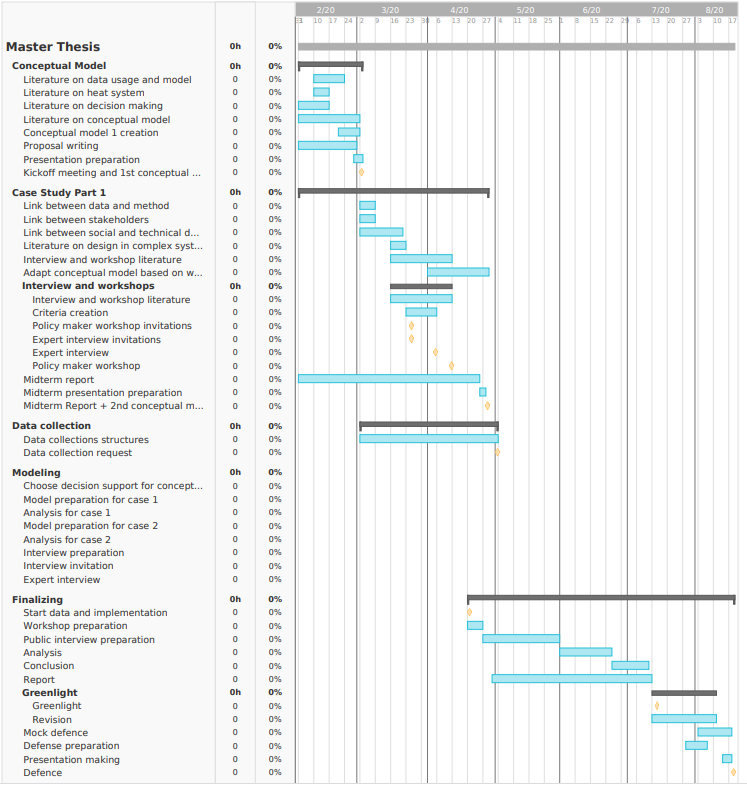
\includegraphics[width=1.2\textwidth]{Images/schedules.PNG}
   \label{fig:schedule}
\end{figure}

Besides this project schedule, a meeting with TNO researchers will be made every Thursday while meetings with the supervisor will be done every second Monday. 








